\chapter{Résultats pour le modèle SOS}

On considère un système de longueur $L$ et de hauteur $N$. Pour $N$ très grand, si la position de l'interface est loin de $0$ ou de $N$, on s'attend à retrouver toutes les propriétés d'un modèle infini centré en 0. Si l'interface est proche de $0$, on pourra étudier les effets au bord, comme dans un système semi-infini\footnote{Dans les simulations numériques ainsi que pour la diagonalisation des matrices nous sommes obligés de choisir une taille finie de notre système. Cependant l'équivalence avec les calculs analytiques dans les sytèmes (semi)infinis mest vraie pour de grandes tailles de systèmes}.  On fixe la hauteur moyenne $<h_i> = H$ grâce au potentiel chimique $\mu$\footnote{Calculer la magnétisation moyenne via des librairies comme \hyperlink{http://eigen.tuxfamily.org/index.php?title=Main_Page}{\underline{Eigen en C++}} (contrairement à la librairie GSL plus difficile d'accès) permet d'accélérer grandement l'étape d'équilibrage du système pour le Monte Carlo.}.

\begin{figure}[h]
	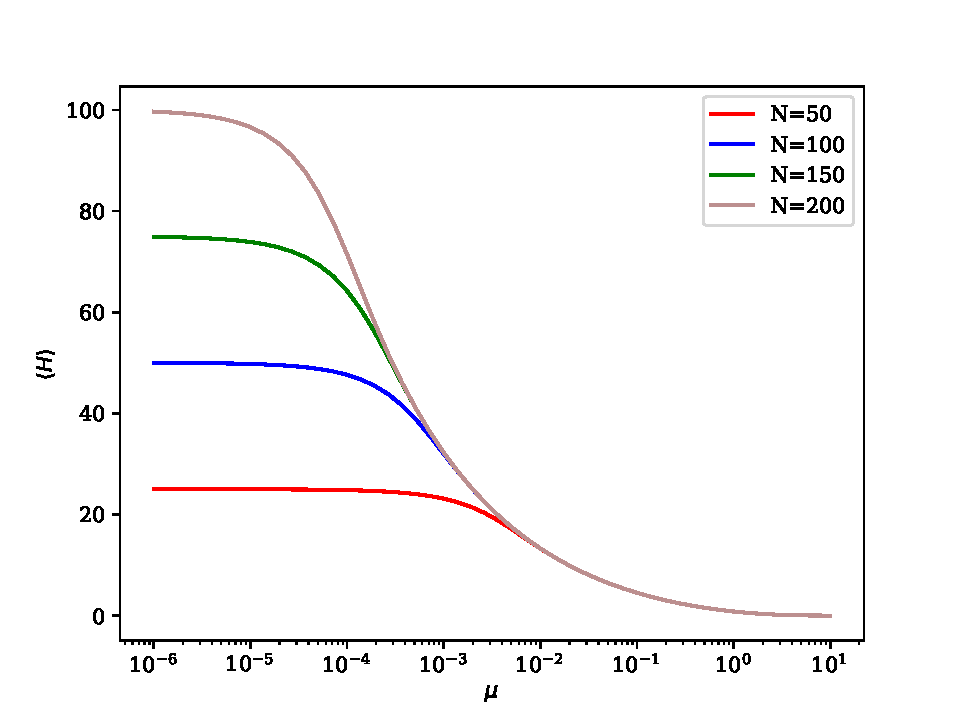
\includegraphics[width=\linewidth]{semiifgeom/hauteur-mu.pdf}
	\caption{Hauteur moyenne de l'hamiltonien $H = \sum_i |h_i-h_{i+1}| + \mu \frac{h_i+h_{i+1}}{2}$ en fonction de $\mu$ calculée grâce à la diagonalisation d'une matrice de transfert de taille $N$. Lorsque le potentiel chimique est trop faible, l'interface est délocalisée et se retrouve à la position $\frac{N}{2}$. }
	\label{hauteur-mu}
\end{figure}

	\section{Différences Glauber/Kawasaki}

figure énergie moyenne, sigma, distribution de probabilité via Airy	
	
	\section{Effet du cisaillement}

Dans les expériences, le système est soumis à un cisaillement au niveau de l'interface, ce qui modifie les observables par rapport à l'état d'équilibre. Nous optons ici pour un modèle de cisaillement uniforme dont le sens est défini par $\sgn(i-j)$, $i$ et $j$ étant des sites de hauteurs respectives $h_i$ et $h_j$. 
La différence d'énergie entre un micro-état et le suivant d'une étape de Monte Carlo sous une dynamique de diffusion (Kawasaki) est alors
\begin{align}
	\Delta E = J \sum_i \left[ |h'_i-h'_{i+1}|-|h_i-h_{i+1}| \right] \pm f 
\end{align}
où $h_i'(t) = h_i(t+1)$ - le temps étant discrétisé, $f$ le module de cisaillement et le signe du cisaillement étant pris de manière aléatoire à chaque étape, regardant ainsi si ce mouvement va dans ou contre le sens du flux. 

Pour rappel, à chaque étape on essaie de transférer une particule du site $i$ vers son voisin (gauche ou droit) $j$, ce qui se traduit par $h_i' = h_i-1$ et $h_j' = h_j+1$. 
Pour $f=0$, en remarquant que les valeurs absolues ont les propriétés suivantes
\begin{align}
	|a \pm 1| - |a| = \pm 1 \\
	|a \pm 2| - |a| = {0,\pm 2}
\end{align}
nous voyons facilement l'émergence d'une sélection des énergies possibles entre deux micro-états successifs dans ${-4,-2,0,2,4}$. Ainsi, toutes les transformations diminuant l'énergie totale du système seront toujours acceptées. En augmentant le cisaillement il devient alors possible de refuser des états réduisant l'énergie et d'accepter ceux qui l'augmente. 
Nous nous attendons alors à trois régimes différents :
\begin{itemize}
	\item $f  \less  2 J $ : à faible cisaillement, la symmétrie du système impose les observables à être paire vis-à-vis de $f$, comme le prouve le fit en carré des figures.
	\item $2 J \less f \less 4 J$ : à cisaillement moyen, certains mouvements augmentant la rugosité de l'interface sont toujours acceptés. 
	\item $f > 4 J$ : à haut cisaillement, tous les mouvements augmentant l'entropie du système sont acceptés. Une saturation du système se produit lorsque l'énergie de lien entre les sites devient négligeable face au cisaillement.
\end{itemize}


\begin{figure}[h]
	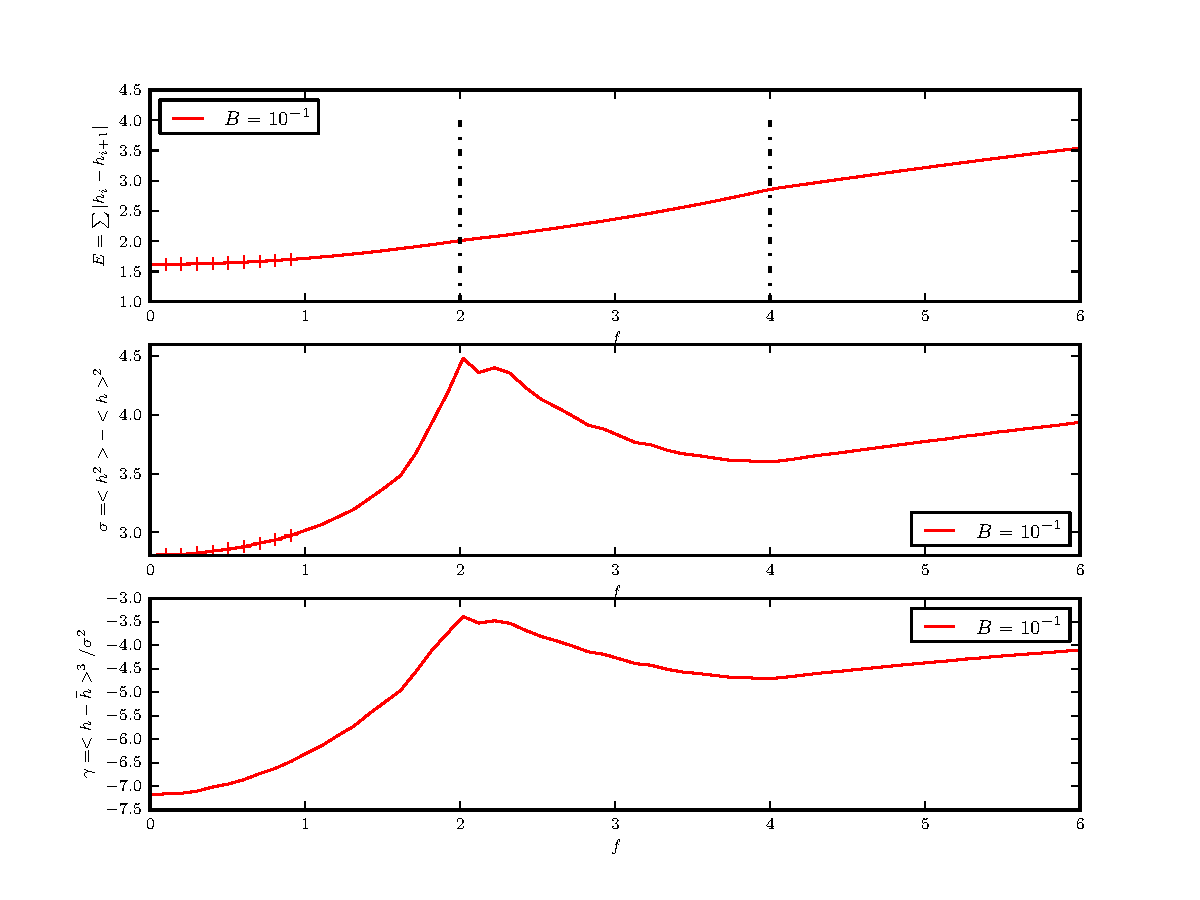
\includegraphics[width=\linewidth]{./semiifgeom/sosj1.pdf}
	\caption{Énergie $E= \langle \sum_i |h_i-h_i+1| \rangle$ (en pointillé sa dérivée), variance $\sigma = \langle (H - \langle H \rangle )^2  \rangle$ et asymétrie $\gamma = \langle (H - \langle H \rangle )^3  \rangle / \sigma^2$ pour $B^0.1$. La magnétisation est constante et égale à $\langle H \rangle = 4.51$. Le temps de corrélation du système est presque constant en fonction du cisaillement $f$, allant de  $\tau(f=0) = 5.04$ à $\tau(f=6) = 5.00$ étapes de Monte Carlo. On note une brisure à $f=2J$ et $f=4J$.
Les croix notent un fit en carré pour petit $f$, montrant la symétrie du système par inversion du signe de $f$. }
\end{figure}

\begin{figure}
	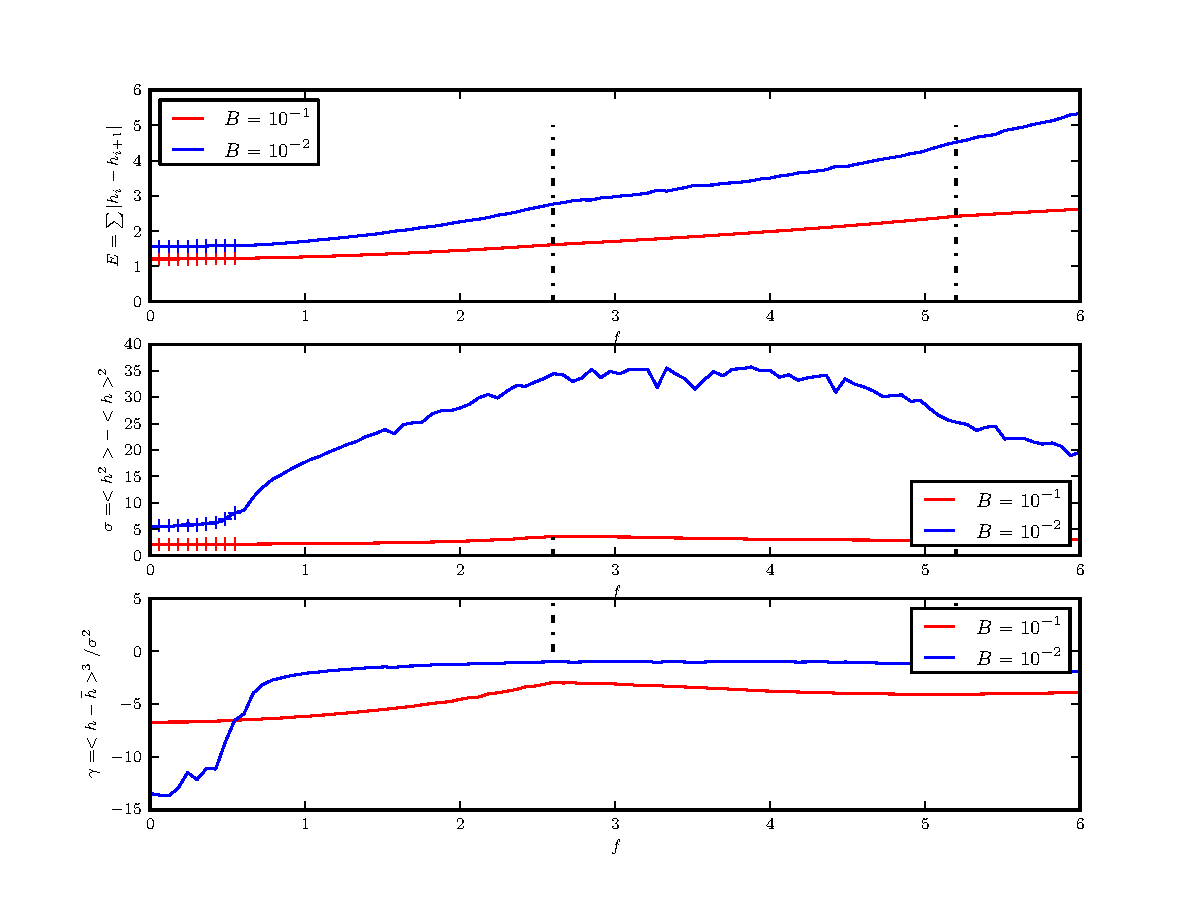
\includegraphics[width=\linewidth]{./semiifgeom/j13.pdf}
	\caption{Same as before, with $J=1.3$ We observe a net inflexion in the energy at $2 J$ for  $B=0.01$ which corresponds to $<H>=11$. Nvertheless there is not threshold at $4 J = 5.2$. My guess is that the system is too far away from the boundary in order to interact strongly with it. Interstingly enough, for $B=0.1$, $<H>=3$ and we are too close to the boundaries to see anything.}
\end{figure}

	\subsection{Différences avec le modèle d'Ising}

	Le modèle d'Ising repose sur la perméabilité entre les deux phases, avec des bulles d'une phase dans l'autre. Dans les travaux sur le rôle du cisaillement au niveau de l'interface dans un modèle d'Ising ( \cite{smith_driven_2010},\cite{smith_interfaces_2008}. ), le cisaillement s'applique à toutes les particules, ce qui a pour but d'étirer les bulles, les rendant plus fragiles au bain thermique. Cet effet participe à leur évaporation vers l'interface et à la dissipation de l'énergie injectée par le cisaillement.
	
	Au contraire, dans les modèles que nous utilisons ici, où l'interface peut fluctuer mais est imperméable, l'énergie injectée au niveau de l'interface ne peut être dissipée par évaporation, ce qui conduit à l'émergence d'une phénoménologie différente. Il est ainsi impossible de définir un cisaillement qui soit appliqué à l'intérieur des phases, puisqu'il n'existe aucune notion de particules. Plus loin nous développons un modèle qui s'abstrait de ces difficultés. 


\section{Cisaillement avec deux types de particules}

La construction naïve d'un modèle continu du cisaillement avec un seul type de particules ne donnera aucun résultat. En effet, pour que le cisaillement induise des effets hors équilibre, il faut que la dynamique des particules dans tout repère galilén soit le même. Si l'on considère une force de cisaillement uniforme qui induit la même vitesse moyenne sur toutes les particules du système, en nous plaçant dans un repère bougeant à la même vitesse que cette vitesse moyenne, nous retrouvons les mêmes propriétés à l'équilibre.
Afin de briser la symmétrie de translation, il faut soit induire un cisaillement non-uniforme, soit introduire des particules qui réagissent de manière différente vis-à-vis de cette force. Dans notre exemple sur les colloïdes, la gravité agit bien sur les polymères mais bien moins sur le solvant, ce qui brise en effet l'invariance galiléenne. 
Plusieurs études récentes portent sur le mouvement de systèmes avec plusieurs particules browniennes\cite{netz2003,dzub2002,chak2003,chak2004,lowe2009,glan2012, klym2016}, incluant le problème des électrolytes étudié par Onsager \cite{onsager} il y a longtemps.

	\subsection{Discussion about the Gaussian model}
	
The Gaussian model has a stronger interaction, been as
\begin{align}
	\Delta E = J \sum (h'_i-h'_{i+1})^2 -(h_i-h_{i+1})^2+ f (i-j)
\end{align}
In this model the bond energy between two microstates can take any integer, as 
\begin{equation*}
	(h_i-h_j+2)^2 - (h_i-h_j)^2 = 4 (h_i-h_j+1)
\end{equation*}

The gaussian interaction is very strong, so we could expect a very smooth interface. The mean difference between two sites should be about $h_i-h_{i+1} \simeq 1$. In that case, the energy difference is discretized as ${-8,-4,0,4,8}$. 
Nonetheless we cannot predict exactly the same behaviour as in the SOS model because this approximation has to be verified everytime, which is false. 1

\begin{figure}
	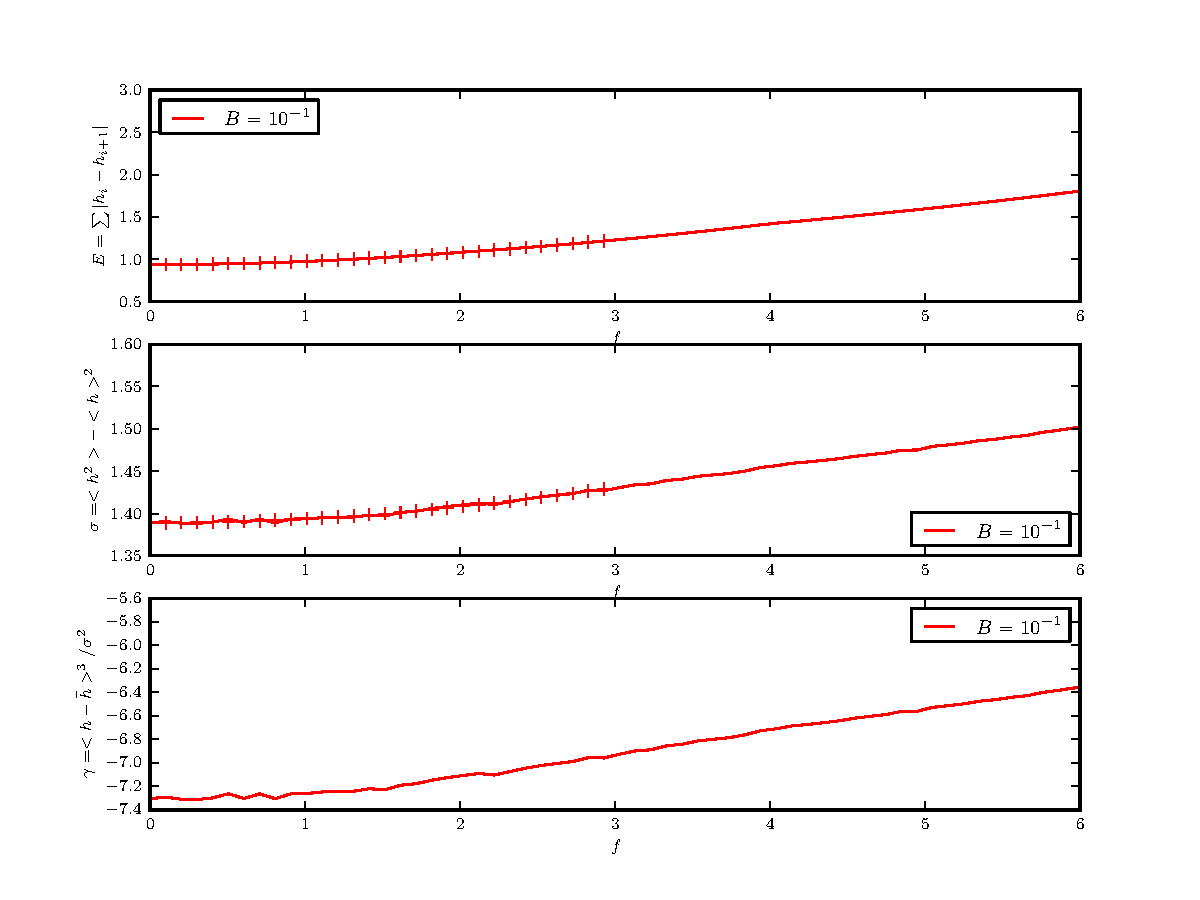
\includegraphics[width=\linewidth]{./semiifgeom/gauss0.pdf}
	\caption{Bond energy, thickness (variance) and skewness of the interface for two different magnetic pressures. The magnetisation is constant and is equal to $<H>=2$ for $B=0.1$. As we are very close to the boundary, we see no threshold with the drive force. Simulations take longer with this model because the interaction is stronger}
\end{figure}

	\section{Interpretation}
	
	